\documentclass[9pt,aspectratio=169]{beamer}
\usepackage{tikz}
\usetheme{Boadilla}
\setbeamertemplate{navigation symbols}{}
\title{Cache invalidation: experiments and bounds}
\subtitle{Generated interaction study}
\author{Research group}
\date{}
\year=2026\month=11\day=5
\newcommand{\fuzzlayerA}[1]{\textit{#1}}
\newcommand{\fuzzlayerB}[1]{\fuzzlayerA{#1}}
\newcommand{\fuzzterm}[1]{\fuzzlayerB{#1}}
\newcommand{\fuzzpair}[2]{\fuzzterm{#1}: #2}
\newcommand{\fuzzunit}{ms}
\let\fuzzoriginalunit\fuzzunit
\newcommand{\fuzzcoefficient}{2}
\newcommand{\fuzzscale}[2][\fuzzcoefficient]{#1\,#2}
\definecolor{fuzzpaint}{RGB}{255,0,255}
\definecolor{fuzzsecond}{RGB}{18,137,67}
\tikzset{fuzzvertex/.style={draw,rounded corners=1pt,fill=blue!10,inner sep=1pt,minimum width=.35cm,minimum height=.25cm}}
\begin{document}
\section{Cache invalidation}
\begin{frame}[t,shrink=5]{Cache invalidation}{Composed dependencies}
\fuzzpair{Experiment}{Timing: 12\fuzzunit; estimate $\fuzzscale{x}+\fuzzscale[2]{y}$.}\par
{\renewcommand{\fuzzunit}{samples}\let\fuzzterm\textbf\fuzzpair{LocalScope}{Timing: 7\fuzzunit.}\par}
\fuzzpair{RestoredScope}{Timing: 11\fuzzunit.}\par
{\footnotesize\color{blue}\raggedright
\begin{description}
\item<1->[Stage 1] \textit{We compare the} proposed solution with a reference computed from the complete input.  The estimate is $\frac{a+b}{1+c}$.
\item<2->[Stage 2] \textbf{A local update} can change the measurements used by several neighboring components.  The estimate is $x_i+x_{i+1}$.
\item<2->[Stage 3] \begin{exampleblock}{Iterative refinement}
\[\begin{pmatrix}a&b\\c&d\end{pmatrix}\begin{pmatrix}x\\y\end{pmatrix}\]
\end{exampleblock}
\end{description}
\par
\begin{description}
\item[Stage 1] \textbf{The next pass} must preserve the boundary conditions while revisiting dependent values.  The estimate is $\frac{a+b}{1+c}$.
\item[Stage 2] \[\begin{aligned}a+b&=c\\ d-e&=f\end{aligned}\]
\item[Stage 3] \only<2-3>{\begin{tabular}{lrr}Method&Cost&Error\\\hline
Fresh0&6&7\\
Fresh1&14&18\\
Global2&5&15\\
\end{tabular}}
\end{description}
\par
\begin{block}{Iterative refinement}
\begin{description}
\item[Stage 1] 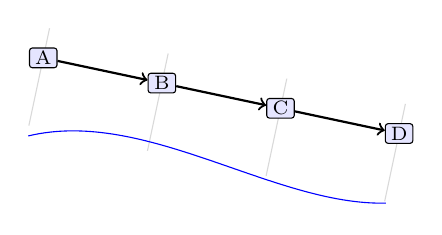
\begin{tikzpicture}[font=\scriptsize]
\begin{scope}[scale=1.1,rotate=-12]

\foreach \x in {0,1,2,3} {\draw[gray!30] (\x*1.400,-.8)--(\x*1.400,.35);}
\node[fuzzvertex] (g15n0) at (0.000,0) {A};
\node[fuzzvertex] (g15n1) at (1.400,0) {B};
\node[fuzzvertex] (g15n2) at (2.800,0) {C};
\node[fuzzvertex] (g15n3) at (4.200,0) {D};
\begin{scope}[xshift=.5pt,yshift=-.5pt]
\draw<2->[->,thick] (g15n0) -- (g15n1);
\draw<2->[->,thick] (g15n1) -- (g15n2);
\draw<2->[->,thick] (g15n2) -- (g15n3);
\draw[blue] (0,-.9) .. controls (1.260,-.3) and (2.940,-1.1) .. (4.200,-.8);
\end{scope}
\end{scope}
\end{tikzpicture}
\item[Stage 2] \textrm{We compare the} proposed solution with a reference computed from the complete input.  The estimate is $x_i+x_{i+1}$.
\item[Stage 3] \begin{enumerate}
\item 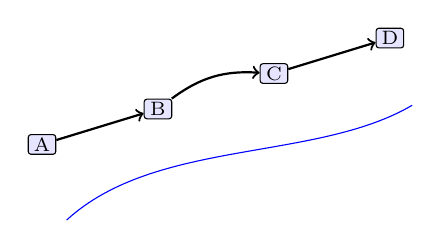
\begin{tikzpicture}[font=\scriptsize]
\begin{scope}[scale=1.1,rotate=17]


\node[fuzzvertex] (g19n0) at (0.000,0) {A};
\node[fuzzvertex] (g19n1) at (1.400,0) {B};
\node[fuzzvertex] (g19n2) at (2.800,0) {C};
\node[fuzzvertex] (g19n3) at (4.200,0) {D};
\begin{scope}[xshift=.5pt,yshift=-.5pt]
\draw<1->[->,thick] (g19n0) -- (g19n1);
\draw<1->[->,thick] (g19n1) to[bend left=20] (g19n2);
\draw<1->[->,thick] (g19n2) -- (g19n3);
\draw[blue] (0,-.9) .. controls (1.260,-.3) and (2.940,-1.1) .. (4.200,-.8);
\end{scope}
\end{scope}
\end{tikzpicture}
\end{enumerate}
\end{description}
\end{block}\par}
\par 
\begin{tikzpicture}[font=\scriptsize]
\fill<2-3>[fuzzpaint] (0,0) rectangle (.8,.3);
\fill<3->[fuzzsecond] (1,0) rectangle (1.8,.3);
\node[anchor=west] at (2,0.15) {Witness};
\end{tikzpicture}
\only<4>{}
\end{frame}
\renewcommand{\fuzzunit}{steps}
\renewcommand{\fuzzcoefficient}{2}
\renewcommand{\fuzzterm}[1]{{\textbf{#1}}}
\section{Iterative refinement}
\begin{frame}[t]{Iterative refinement}
\fuzzpair{MacroStageB}{Timing: 12\fuzzunit, retained: 9\fuzzoriginalunit.}\par
{\renewcommand{\fuzzunit}{local}\fuzzpair{FrameLocal}{Timing: 5\fuzzunit.}\par}
\fuzzpair{FrameRestored}{Timing: 8\fuzzunit; estimate $\fuzzscale{x}$.}\par
\begin{columns}[T]\begin{column}{.46\textwidth}A local update can change the measurements used by several neighboring components.\end{column}\begin{column}{.46\textwidth}\begin{itemize}\item Input state\item Updated state\end{itemize}\end{column}\end{columns}
\end{frame}
\renewcommand{\fuzzunit}{min}
\renewcommand{\fuzzcoefficient}{3}
\renewcommand{\fuzzterm}[1]{{\textit{#1}}}
\section{Message passing}
\begin{frame}[t]{Constraint propagation}
\fuzzpair{MacroStageC}{Timing: 12\fuzzunit, retained: 9\fuzzoriginalunit.}\par
{\renewcommand{\fuzzunit}{local}\fuzzpair{FrameLocal}{Timing: 5\fuzzunit.}\par}
\fuzzpair{FrameRestored}{Timing: 8\fuzzunit; estimate $\fuzzscale{x}$.}\par
\begin{block}{Follow-up}\fuzzterm{A revised value} depends on the preceding frame.\end{block}
\[r_{k+1}=r_k-\alpha d_k\]
\end{frame}
\end{document}
